\documentclass[master,proposal,extern,palatino]{rgseThesis}



% für "lorem ipsum" Blindtext - sollte bei echten Arbeiten natürlich raus ;-)
\usepackage{lipsum}
\usepackage{enumitem}
\usepackage{comment}
\newcolumntype{Y}{>{\centering\arraybackslash}X}
\newcommand{\mycomment}[1]{}



% Angaben für die Titelseite
\author{Gadiyaram, Sri Sai Praveen}
% \studiengang{Web and Data Science} % Default ist Informatik, bei Proposals ignoriert

\title{Sub-topic modeling and ranking analysis in document retrieval systems}

\supervisor{w}{Prof. Dr. Jan Jürjens} % Default ist Jan Jürjens
\supervisorInfo{Institute for Software Technology} % Default ist Institut für Softwaretechnik

\secondSupervisor{w}{MSc. Katharina Großer}
\secondSupervisorInfo{Institute for Software Technology}

\externLogo{7cm}{logos/fkie} % optional Logo des externen Partners
\externName{Informationstechnik für Führungssysteme (ITF)} % optional Untertitel des Logos

\usepackage[backend=biber]{biblatex}
% Literatur-Datenbank
\addbibresource{literature.bib}

% Tiefe des Inhaltsverzeichnisses; 1: bis section (empfohlen), 2: bis subsection
\setcounter{tocdepth}{2} 

\begin{document}

% Umschalten der Sprache für englische Rubrikbezeichnungen (möglich: english, ngerman)
\selectlanguage{english}
\setlength{\parindent}{20pt}

% Titelseite
\maketitle

% Inhaltsverzeichnis
\tableofcontents

% Hier kommt jetzt der eigentliche Text des Proposals
	\pagebreak

\section{Introduction}


Retrieving highly relevant documents in the top results for a given user query is one of the challenging tasks in Information Retrieval (IR). This challenge is amplified when the user has a specific intention, and the search query lacks the context of their intention. For example, the user query \textit{"Robotics"} can retrieve documents related to many domains such as manufacturing, agriculture, military, etc. A simple keyword search can overwhelm the user with many false positives when the user wants to explore the innovation documents only related to a specific domain, such as \textit{"Military"}. To fulfill the user intent and missing context in the user query, a novel  document modeling approach for retrieval is proposed to extract highly coherent query-specific contexts (sub-topics) from the top retrieved documents, which helps the user immensely to narrow down the search space. Furthermore, the proposed approach will be evaluated using precision and survey analysis.

	\section{Research Questions (RQ)}

An unsupervised soft clustering approach is proposed to model documents (from multiple
languages) as a mixture of sub-topics, which are extracted using the deep inherent information
from keywords. Below are the research questions that address the problem mentioned above through a new document modeling approach.

\paragraph{RQ1:} \textbf{ \textit{How effective is the sub-topic modeling approach in creating distinctive clusters from the news articles?}}

This research question aims to test the effectiveness of the above-proposed approach. Both intrinsic and extrinsic clustering evaluation techniques, as well as a survey, are chosen to evaluate the clustering output.

\paragraph{RQ2:} \textbf{ \textit{Which IR system retrieves more relevant documents for a user query and a sub-topic? }}

When a user chooses a particular sub-topic cluster, it is assumed that the retrieval results related to the query and the sub-topic are shown. Two different IR  systems are proposed in this master thesis to retrieve documents relevant to both the given user query and the chosen sub-topic. This research question targets comparing these two retrieval systems and determining the better one. A survey will be performed, and the collected data will be analyzed to answer the  \textit{RQ2}


\paragraph{RQ3:} \textbf{ \textit{What is the effect of sub-topic ranking in finding the positive documents from the candidate pool? }}

Showing only the documents related to a specific sub-topic can restrict the user from viewing
the original retrieved results for the given query. This research question addresses the impact
of the sub-topic clustering output to find the positive documents against the baseline approach
and is evaluated through an exploratory precision analysis. 

\section{Background and Motivation}

	\subsection{Fraunhofer FKIE}
	
	Fraunhofer FKIE (Fraunhofer-Institut für Kommunikation, Informationsverarbeitung und Ergonomie) is a research institute for providing innovative solutions in information and communications technology, and their main focus is on developing effective and efficient human-machine systems\footnote{\url{https://www.fkie.fraunhofer.de/en/about-fkie.html}}. The users at FKIE are especially interested in reading news articles related to innovation and breakthroughs in \textit{Technology and Military}. The below image, \prettyref{fig:areas_of_interest}, shows an example of areas of interest to the FKIE users, and this list is not bounded and can include more domains.

	\begin{figure}[h]
		\centering
		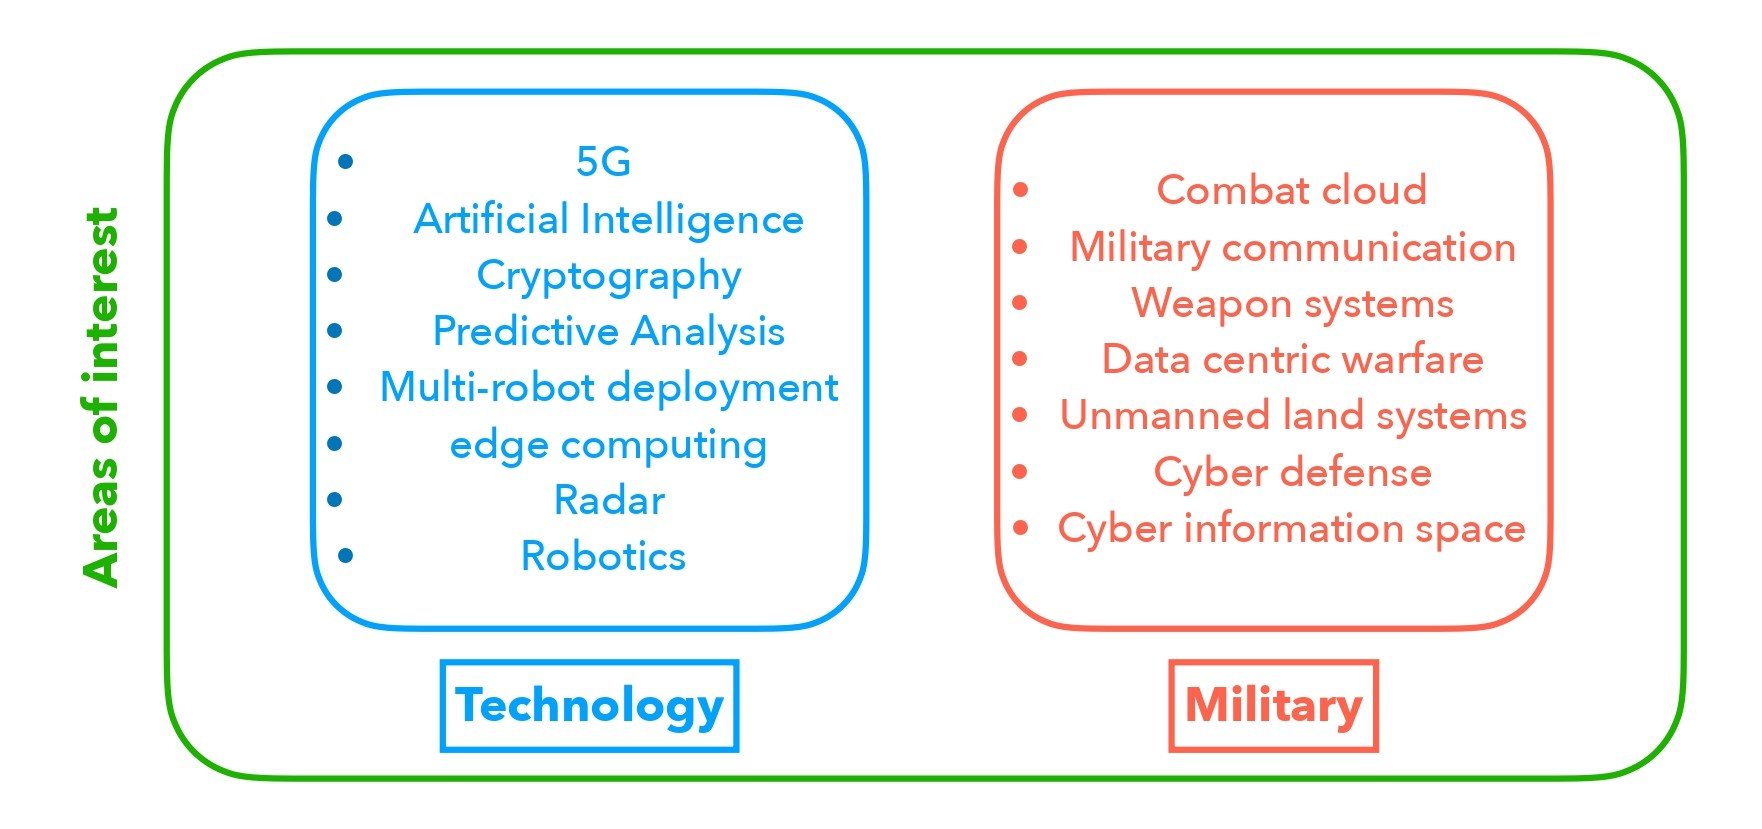
\includegraphics[width=.7\textwidth]{images/keynotes_images/areas_of_interest.jpg}
		\caption{Areas of interest for the users at FKIE \label{fig:areas_of_interest}}
	\end{figure} 

\subsection{Technical details}
\subsubsection{Abbreviations}

\begin{enumerate}
	\item{\textbf{URL:}} A URL is a short form for \textit{Uniform Resource Locator} and is used to locate resources uniquely on the Internet~\cite{berners1994uniform}. Any resource on the Internet can be accessed with a unique URL. For example, the URL <https://www.linux.org/> represents a resource on the Internet. 

	\item{\textbf{HTML:}} HTML stands for \textit{HyperText Markup Language} and is a markup language for representing documents on the World Wide Web (WWW) and links to other documents or information sources such as images, video, audio, etc~\cite{html}.
\end{enumerate}	


\subsubsection{Machine Learning (ML)}

\begin{enumerate}
	
\item{\textbf{Ground-truth:}} Ground-truth labels are the information that is more accurate, relevant, and true than the knowledge of the system we are testing~\cite{cardoso2014gold}. This information is critical to evaluate and compare different systems.

\item{\textbf{Supervised learning:}} Supervised learning algorithms are ML approaches that use labeled data~\cite{9155761} for training the algorithm parameters using specific criteria or a loss function. \textit{Classification} is a supervised technique to learn patterns from the labeled data and classify the unseen data automatically into several classes. 
   
\item{\textbf{Unsupervised learning:}} Clustering is an example
of these algorithms, and similar data points are clustered into groups according to the
features in the data~\cite{mahesh2020machine}. These groups are called \textit{Clusters}. Document clustering is a technique to group documents into topics without ground-truth information~\cite{de2012document}.

\item{\textbf{Soft clustering:}} In \textit{Soft clustering}, the data points are assigned to one or more clusters by the clustering algorithm~\cite{de2012document}. This depends mainly on the structure of the data, and especially in news articles, documents are assigned to multiple topics rather than one.

\item{\textbf{Support Vector Machine (SVM):}} SVM is a supervised learning algorithm used for classification and regression. Using the labeled data information, \textit{SVM} selects a maximum margin separating hyperplane(a decision boundary) between the data points. This hyperplane is used later for classifying new data points~\cite{noble2006support}. 

\item{\textbf{Tensorflow Hub:}} Tensorflow Hub\footnote{\url{https://www.tensorflow.org/hub}} is a repository of pre-trained ML models from \textit{Tensorflow}\footnote{\url{https://www.tensorflow.org/}}. Tensorflow is an open-source platform for ML that provides an ecosystem of
tools and libraries and allows developers to build and deploy ML-powered apps and
researchers to push state-of-the-art models~\cite{tensorflow_developers_2022_6574269}. 

\end{enumerate}	

\subsubsection{Natural Language Processing (NLP)}

\begin{enumerate}
	
	\item{\textbf{Token:}} In NLP, a token is a word or basic entity in a text document, and Tokenization is the
	process of splitting a text document into tokens~\cite{webster1992tokenization}. Document token length is calculated as the number of tokens present in a document.
	
	\item{\textbf{Noun chunks:}} Noun chunks or phrases are the nouns and all the words that depend on these nouns~\cite{noun_chunk}. Consider the sentence, \textit{"Army project may improve military communications by boosting 5G technology"}~\cite{sample_news_article}. The possible noun chunks extracted from this sentence are \textit{"Army project", "Military communications", "5G technology"}.
	
	\item{\textbf{Keywords:}} Keywords are the noun chunks that are highly meaningful in a text document and can best describe or summarize a document~\cite{beliga2014keyword}. An unsupervised multi-lingual keyword extraction approach is used in the proposed approach to extract the most significant keywords from each news article.
	
	\item{\textbf{Sentence embeddings:}} The distributed vector representation of a sentence or paragraph
	in a semantic space is generally referred to as sentence embeddings. These embeddings can
	also be generated with short phrases and noun chunks~\cite{cer2018universal, yang2019multilingual}.
	
	\item{\textbf{Universal sentence encoder (USE):}} USE is an ML model that encodes text data such as
	sentences, phrases, or paragraphs into a distributed semantic vector. USE embeds text from
	sixteen different languages into a single semantic space~\cite{cer2018universal, yang2019multilingual}. In this master thesis, a USE model from Tensorflow Hub\footnote{\url{https://tfhub.dev/google/universal-sentence-encoder-multilingual-large/3}} is used. 
	
	\item{\textbf{Lexical matching:}} Lexical or syntactic matching is a technique to assign a relevance score between two text data (strings) based on the terms present in the data. This matching technique is not optimal for retrieval, as it does not consider the meaning of the query  ~\cite{kuzi2020leveraging}.
	
	\item{\textbf{Semantic matching:}} Semantic matching assigns a relevance score between the two text
	data by considering the semantic information (meaning of the terms).

\end{enumerate}	

\subsubsection{Information Retrieval (IR)}

\begin{enumerate}
	\item{\textbf{Document retrieval system:}} IR system specially developed to retrieve the document or
	text data for a given user query is generally referred to as a Document retrieval system.
	
	\item{\textbf{BM-25:}} BM-25, Best Match 25, is a ranking function based on a probabilistic
	relevance framework that ranks documents based on the query terms occurring in each
	document~\cite{amati_bm25_2009}. BM-25 ranking is a lexical or syntactic matching approach and does not consider word semantics. 
	
	\item{\textbf{Semantic search:}} Unlike syntactic matching or calculating term frequencies, Semantic
	search engines try to understand the meaning of the search query and retrieve the
	matching documents close to the query in the semantic space~\cite{dong2008survey}.
\end{enumerate}	

\subsubsection{Data storage}

\begin{enumerate}
	\item{\textbf{Document index:}} Document indexing or compression is a technique to store documents in an optimized way on the disk for efficient retrieval. This stored data on the disk is now
	referred to as \textit{Document Index}~\cite{ziviani2000compression}. 
	
	\item{\textbf{Inverted index:}}   The \textit{Inverted index} is a data structure that contains every word in the corpus and the separate list of documents where the word occurs~\cite{ziviani2000compression}. 
	
	\item{\textbf{Semantic search index:}} The \textit{Semantic search index} stores the distributed embedding vectors of the documents on the disk and uses them later for retrieval.
	 
	\item{\textbf{SQLite DB:}} SQLite is a lightweight serverless, self-contained, transactional database engine~\cite{bhosale2015sqlite}. In this master thesis, labeled data are stored in \textit{SQLite DB} using a library \textit{sqlite3}\footnote{\url{https://docs.python.org/3/library/sqlite3.html}}.
	
\end{enumerate}	

\subsubsection{Evaluation}

\begin{enumerate}
	
	\item{\textbf{Intrinsic evaluation:}} In case of no labeled data or ground-truth, the clustering output is evaluated through the methods considering only the inherent representation of clustered data~\cite{de2012document}. These methods of evaluation are referred to as \textit{Intrinsic evaluation}. 
	
	\item{\textbf{Extrinsic evaluation:}} In \textit{Extrinsic evaluation}, the clustering output is evaluated using the external knowledge such as ground-truth or the relevance judgments~\cite{de2012document}. 
	
	\item{\textbf{Silhouette index:}} Irrespective of the clustering algorithm, the output is more distinctive when
	the distance between the data points within the cluster is minimum and the distance between
	the clusters is maximum. Silhouette index~\cite{rousseeuw1987silhouettes} is an intrinsic clustering evaluation measure and is calculated by using the intra-cluster and inter-cluster distances for each sample. 
 
	\item{\textbf{Precision:}} In IR system evaluation, \text{Precision} is defined as the ratio of retrieved documents that are relevant to all the retrieved documents~\cite{zuva2012evaluation}. This measure can be used to compare different IR systems and be calculated at different retrieved indices. For example, $P@5, P@10, P@15$ measures precision scores at retrieved indices $5, 10, 15$ respectively.
	
	\item{\textbf{Cosine similarity:}} Cosine similarity is a metric to measure the degree of similarity between two vectors~\cite{lahitani2016cosine}. In the case of IR systems, the similarity is calculated between the user query and document sentence embeddings, and can be further used to rank the documents.
	 
\end{enumerate}	


\subsubsection{Keywords specific to this master thesis}

\begin{enumerate}
	
	\item{\textbf{News article:}} A news article is a text document published by a news website.  An example of a news article (this is only a part of the original article) is shown in \prettyref{fig:sample_newsarticle}.
	
	\begin{figure}[h]
		\centering
		
\includegraphics[width=.8\textwidth]{images/mitera_screenshots/sample_news_article.PNG}
		\caption{A sample news article from the document database~\cite{sample_news_article}\label{fig:sample_newsarticle}}
	\end{figure} 
	
	
	
	\item{\textbf{Web scraping:}} Web scraping is a technique to automatically extraction of  data from websites~\cite{khder2021web}. In the case of text data, most approaches download the structured HTML webpages and extract needed information. In this master thesis, news articles from different websites are scraped.
	
	\item{\textbf{Candidate pool:}} A candidate or retrieval pool is a set of documents from lexical and
	semantic matching results for a given user query. These documents are very diverse, contain keywords present in the query (or semantically similar), and are further used for
	clustering.
	  
	\item{\textbf{Sub-topic:}} Sub-topics are second-level representations of a document. Generally, news
	articles are long text documents and can not be represented logically with a single
	topic or keyword. If the user query provided to the \textit{Retriever} is considered the main topic, then the distinctive topics extracted from the candidate pool are sub-topics.
	
	\item{\textbf{Context:}} In this master thesis, we define a context as a particular domain or field in which
	the user is interested. For example, in the user query \textit{Cloud}, the retrieved documents are
	related to different domains or contexts, such as cloud computing, combat cloud, and clouds
	in the sky. Even though there is some syntactic and semantic matching, the user intention is still unclear from the query. 	
	
	\item{\textbf{Labeler:}} A person who assigns an appropriate label to the data according to the labeling criteria.
	
	\item{\textbf{Query type:}} Input search queries from the user can be of any form. For example ., abbreviation, single word query, etc. In this master thesis, each form of a possible user query is referred to as a query type. All possible user queries can be categorized into two major query types, namely phrase (three words or less) and sentence queries.
	
\end{enumerate}	


\subsection{Background and retrieval setup}

A document retrieval system was developed to support users at FKIE in retrieving news articles  related to technology and military topics. The retrieval setup contains three primary components:  \textit{Web scraper, Document filter}, and \textit{Retriever}, as shown in \prettyref{fig:background_image}. The first component, the \textit{Web scraper}, downloads news articles (HTML pages) from a list of URLs and cleans the raw HTML
data from advertisements and noise. Each cleaned news article is considered as a single entity, namely a \textit{Document}. The majority of  downloaded documents are a mixture of topics such as military, technology, artificial intelligence, etc., and also contain a small number of typical news topics, namely politics, sports, advertisements, etc. The downloaded news articles are in \textit{German} and \textit{English}.

\begin{figure}[h]
	\centering
	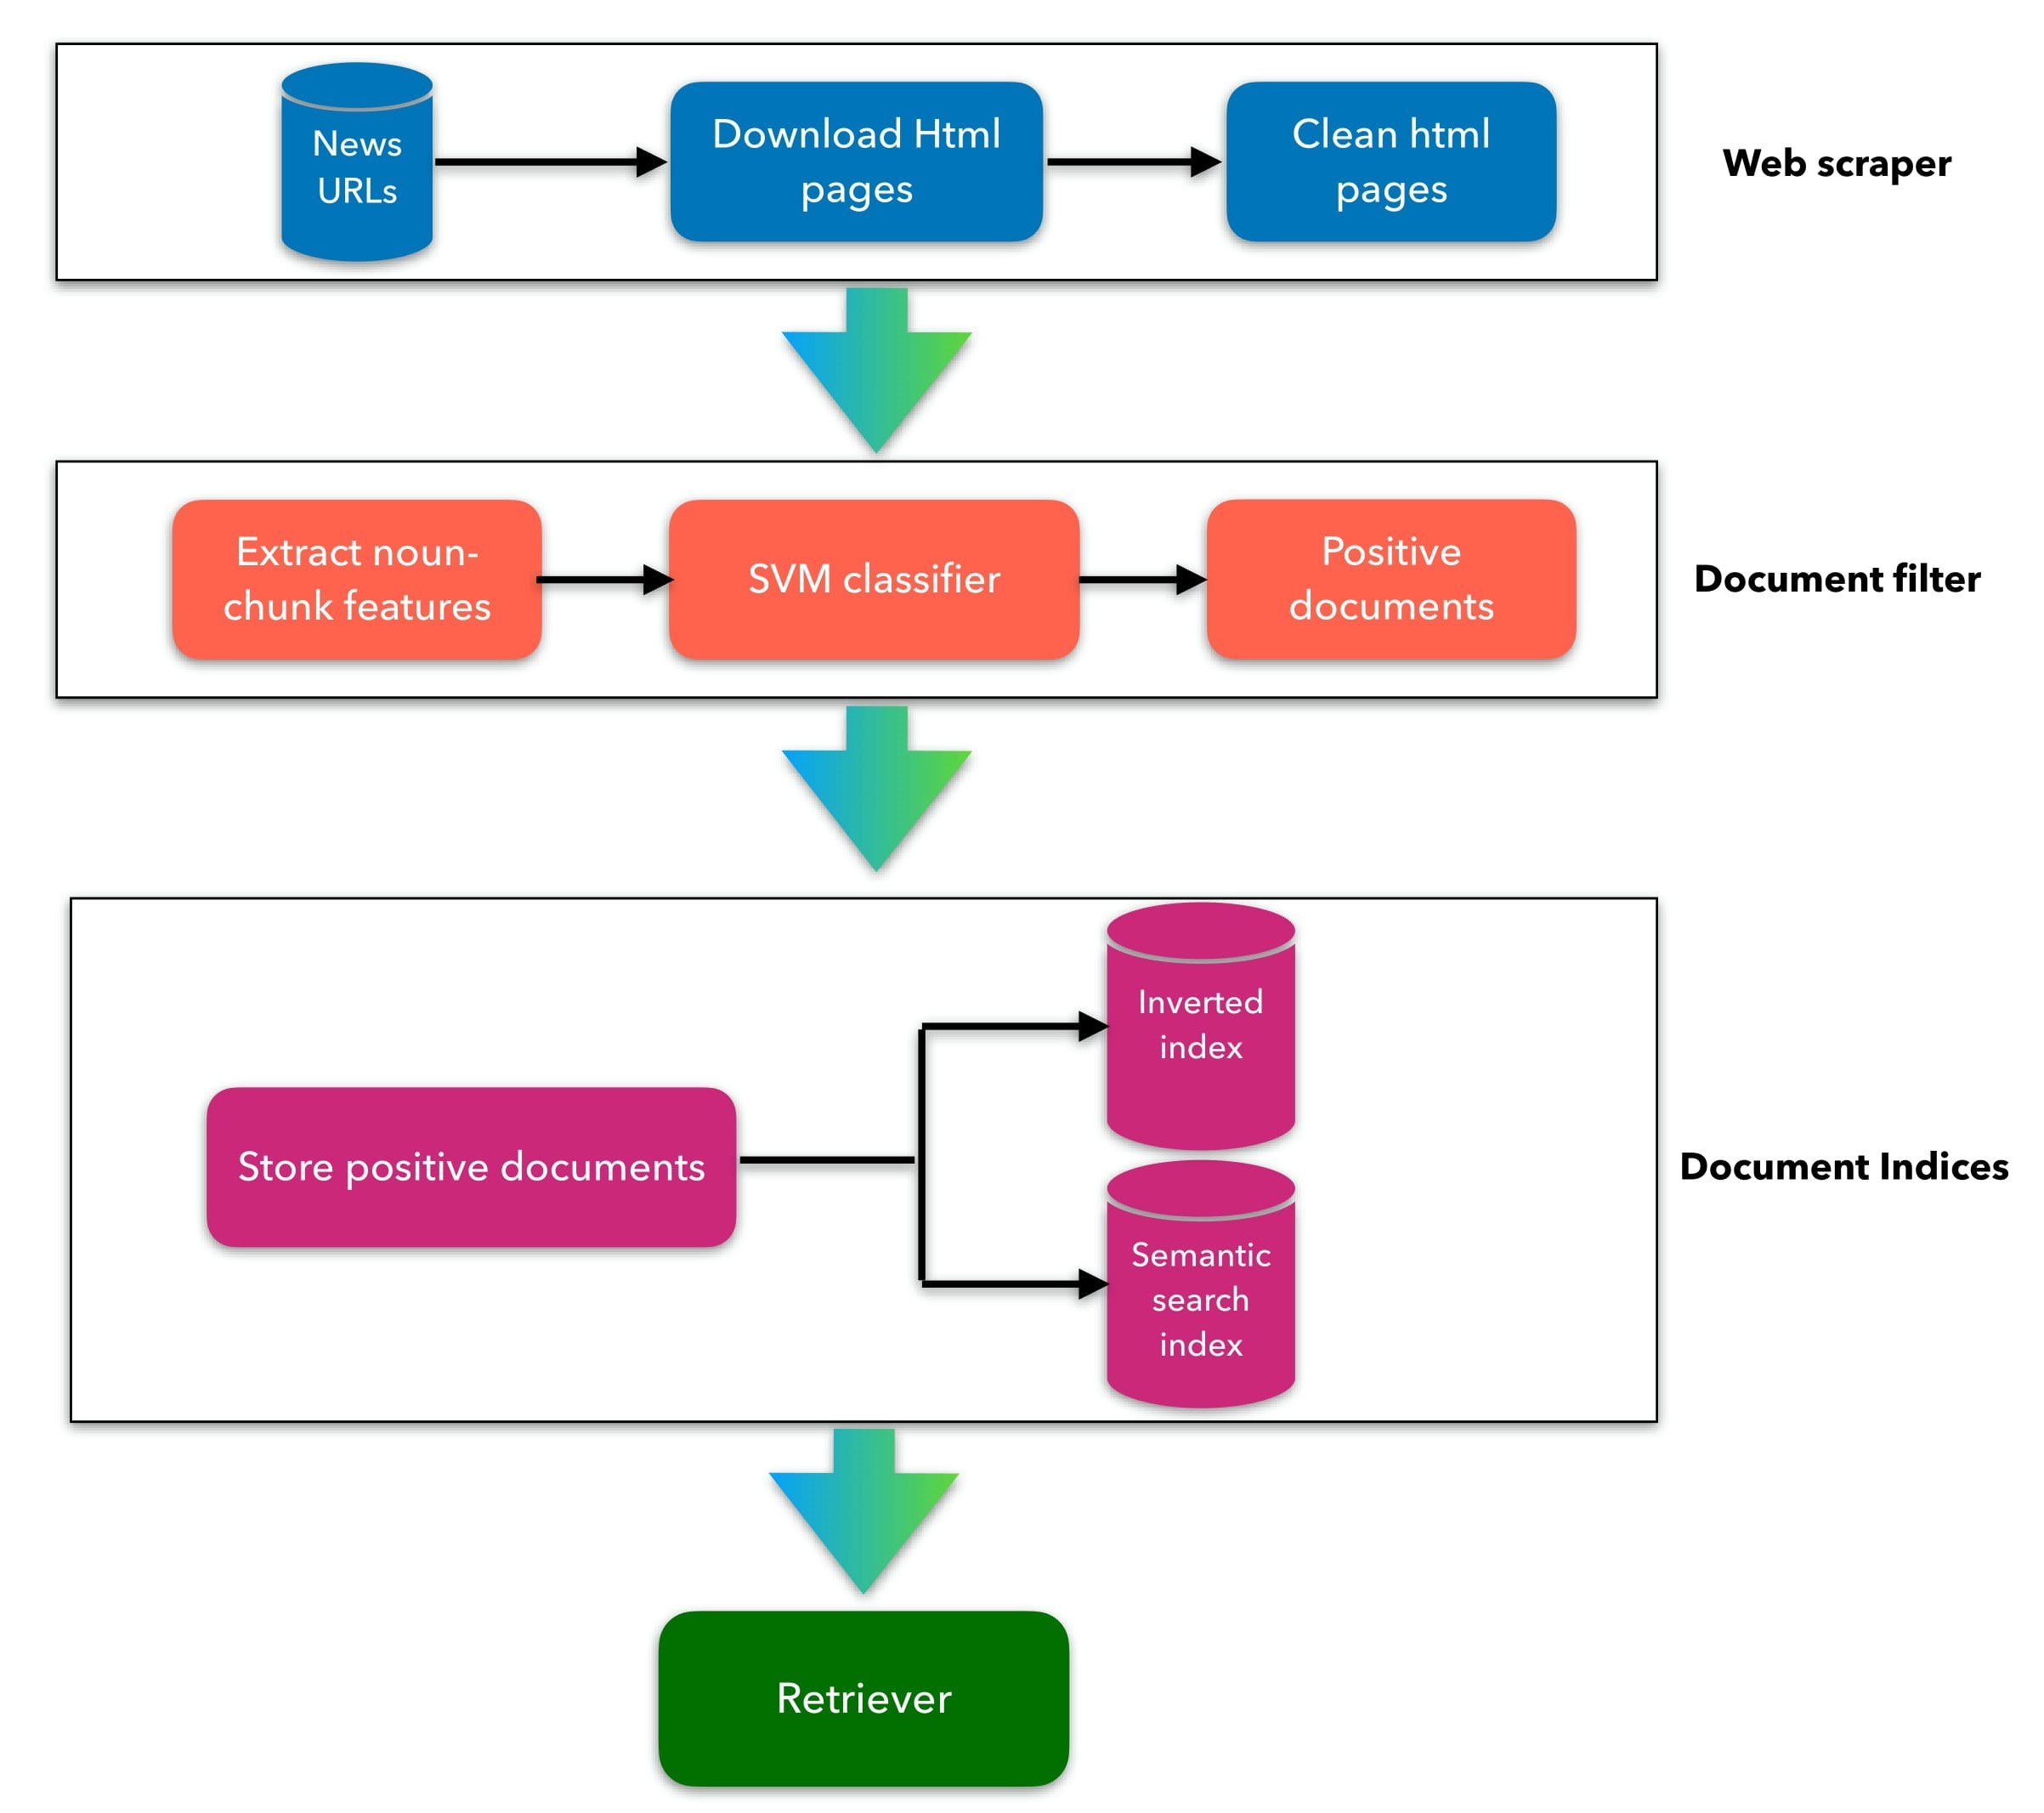
\includegraphics[width=.8\textwidth]{images/keynotes_images/background.jpg}
	\caption{Document retrieval system designed at Fraunhofer FKIE \label{fig:background_image}}
\end{figure}

The second component, the \textit{Document filter}, is based on Support Vector Machine (SVM) classifier that filters most of the irrelevant documents related to specific news topics. The documents are classified into two classes namely, \textit{Positive} and \textit{Negative}. \textit{Positive} documents are documents related to technology and military, and \textit{Negative} documents are related to everything else. After several tests at FKIE, it was found that features from noun-chunks in a document are performing better to differentiate \textit{Positive} documents from the \textit{Negative} documents. Noun chunk features based on the pre-trained multi-lingual Universal Sentence Encoder (USE) is used for the task of classification. 

\begin{figure}[h]
	\centering
	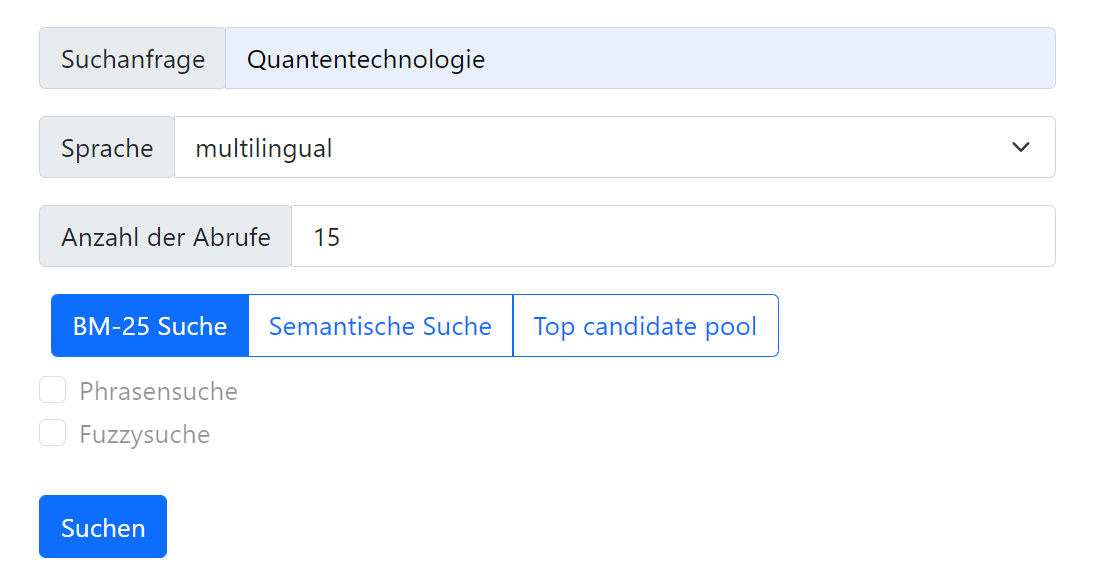
\includegraphics[width=.8\textwidth]{images/mitera_screenshots/newsfeeds_search.PNG}
	\caption{User interface to retrieve documents for FKIE users \label{fig:mitera_search}}
\end{figure}

In order to facilitate positive documents to the FKIE users, a \textit{Retriever} component is designed to retrieve documents for a given user query using lexical and semantic matching techniques.   Therefore, the positive documents from the \textit{Document filter} stage are stored in two different document indices namely \textit{Inverted index} and \textit{Semantic search index}. Finally, the component \textit{Retriever} uses both of the indices and retrieves documents according to the user request through a web user interface, as shown in \prettyref{fig:mitera_search}.

 
\subsection{Challenges}

 Semantic matching of query and documents is better suited when the user query is a long sentence query due to the context embedded in the search query. For example, the user query \textit{"What are the technological advancements in Robotics related to Unmanned Weapon Systems?"} provide high-quality results in the top results, as the information request is detailed in the query. Consequently, the search query  \textit{"Robotics"} results are mapped to multiple domains and lead to many false positives (according to the user's intention). 
 
 \begin{center}
 	\captionof{table}{Retrieval algorithms comparison on different query types}\label{tab:ir_system_comparison}
 	\begin{tabularx}{.99\textwidth}{|c|Y|Y|Y|Y|}
 		
 		\hline
 		S No. &  Query type & Better retrieval technique &  Reason &  Queries used  \\
 		\hline
 		1 & No meaning queries & BM-25 &  Lexical matching  & Person or object names\footnote{User query with no innate meaning of the word namely out of vocabulary words: for example John Dowe, Wester etc.} \\
 		\hline
 		2 & Multi-lingual queries & Semantic search &  Semantic matching & Artificial Intelligence vs Künstliche Intelligenz\\
 		\hline
 		3 & German composite words  & Semantic search&  Semantic matching & Quantentech- nologie \\
 		\hline
 		4 & Spelling mistakes  &  Semantic search&  Semantic matching & Kryptografy, Rbot \\
 		\hline
 		5 & Polysemy  & Semantic search&  Semantic matching & Combat Cloud, Cloud computing \\
 		\hline
 		6 & Sentence/long phrase queries  & Semantic search&  Semantic matching  & Schwachstell-
 		enanalyse eigene Waffen-Systeme \\
 		\hline
 		
 	\end{tabularx}
 \end{center}
 
 
 In the case of keyword queries, it was observed that semantic and lexical matching are prone to high false positives and have no unique advantage. In ~\cite{kuzi2020leveraging}, the authors observed a similar challenge in their research.
 On the one hand, lexical matching does not consider the inherent meaning of the word causing a vocabulary
 mismatch problem, and semantic matching fails to retrieve the relevant documents in the
 top results as it matches too many keywords semantically. A manual observation of retrieved results is carried out with a set of sample queries to evaluate the retrieval algorithms, and the results are shared in \prettyref{tab:ir_system_comparison}. 


The users at FKIE provide only one or two phrase queries, and his or her intention is to explore information to specific topics such as \textit{"Technology"} and \textit{"Military"}. Without labeled data, learning user intention from a single word or phrase query is a huge challenge.  One further challenge is that a wide variety of sources can also result in high noise or false positives, and the user is less likely to find the relevant documents in the top results. Unlike tweets or requirements, news articles are long documents with the $50\%$ (percentile) token length of 788 and consist of keywords from multiple domains. Document token length details is shown in \prettyref{fig:token_length_distribution}. 

 \begin{figure}[h]
	\centering
	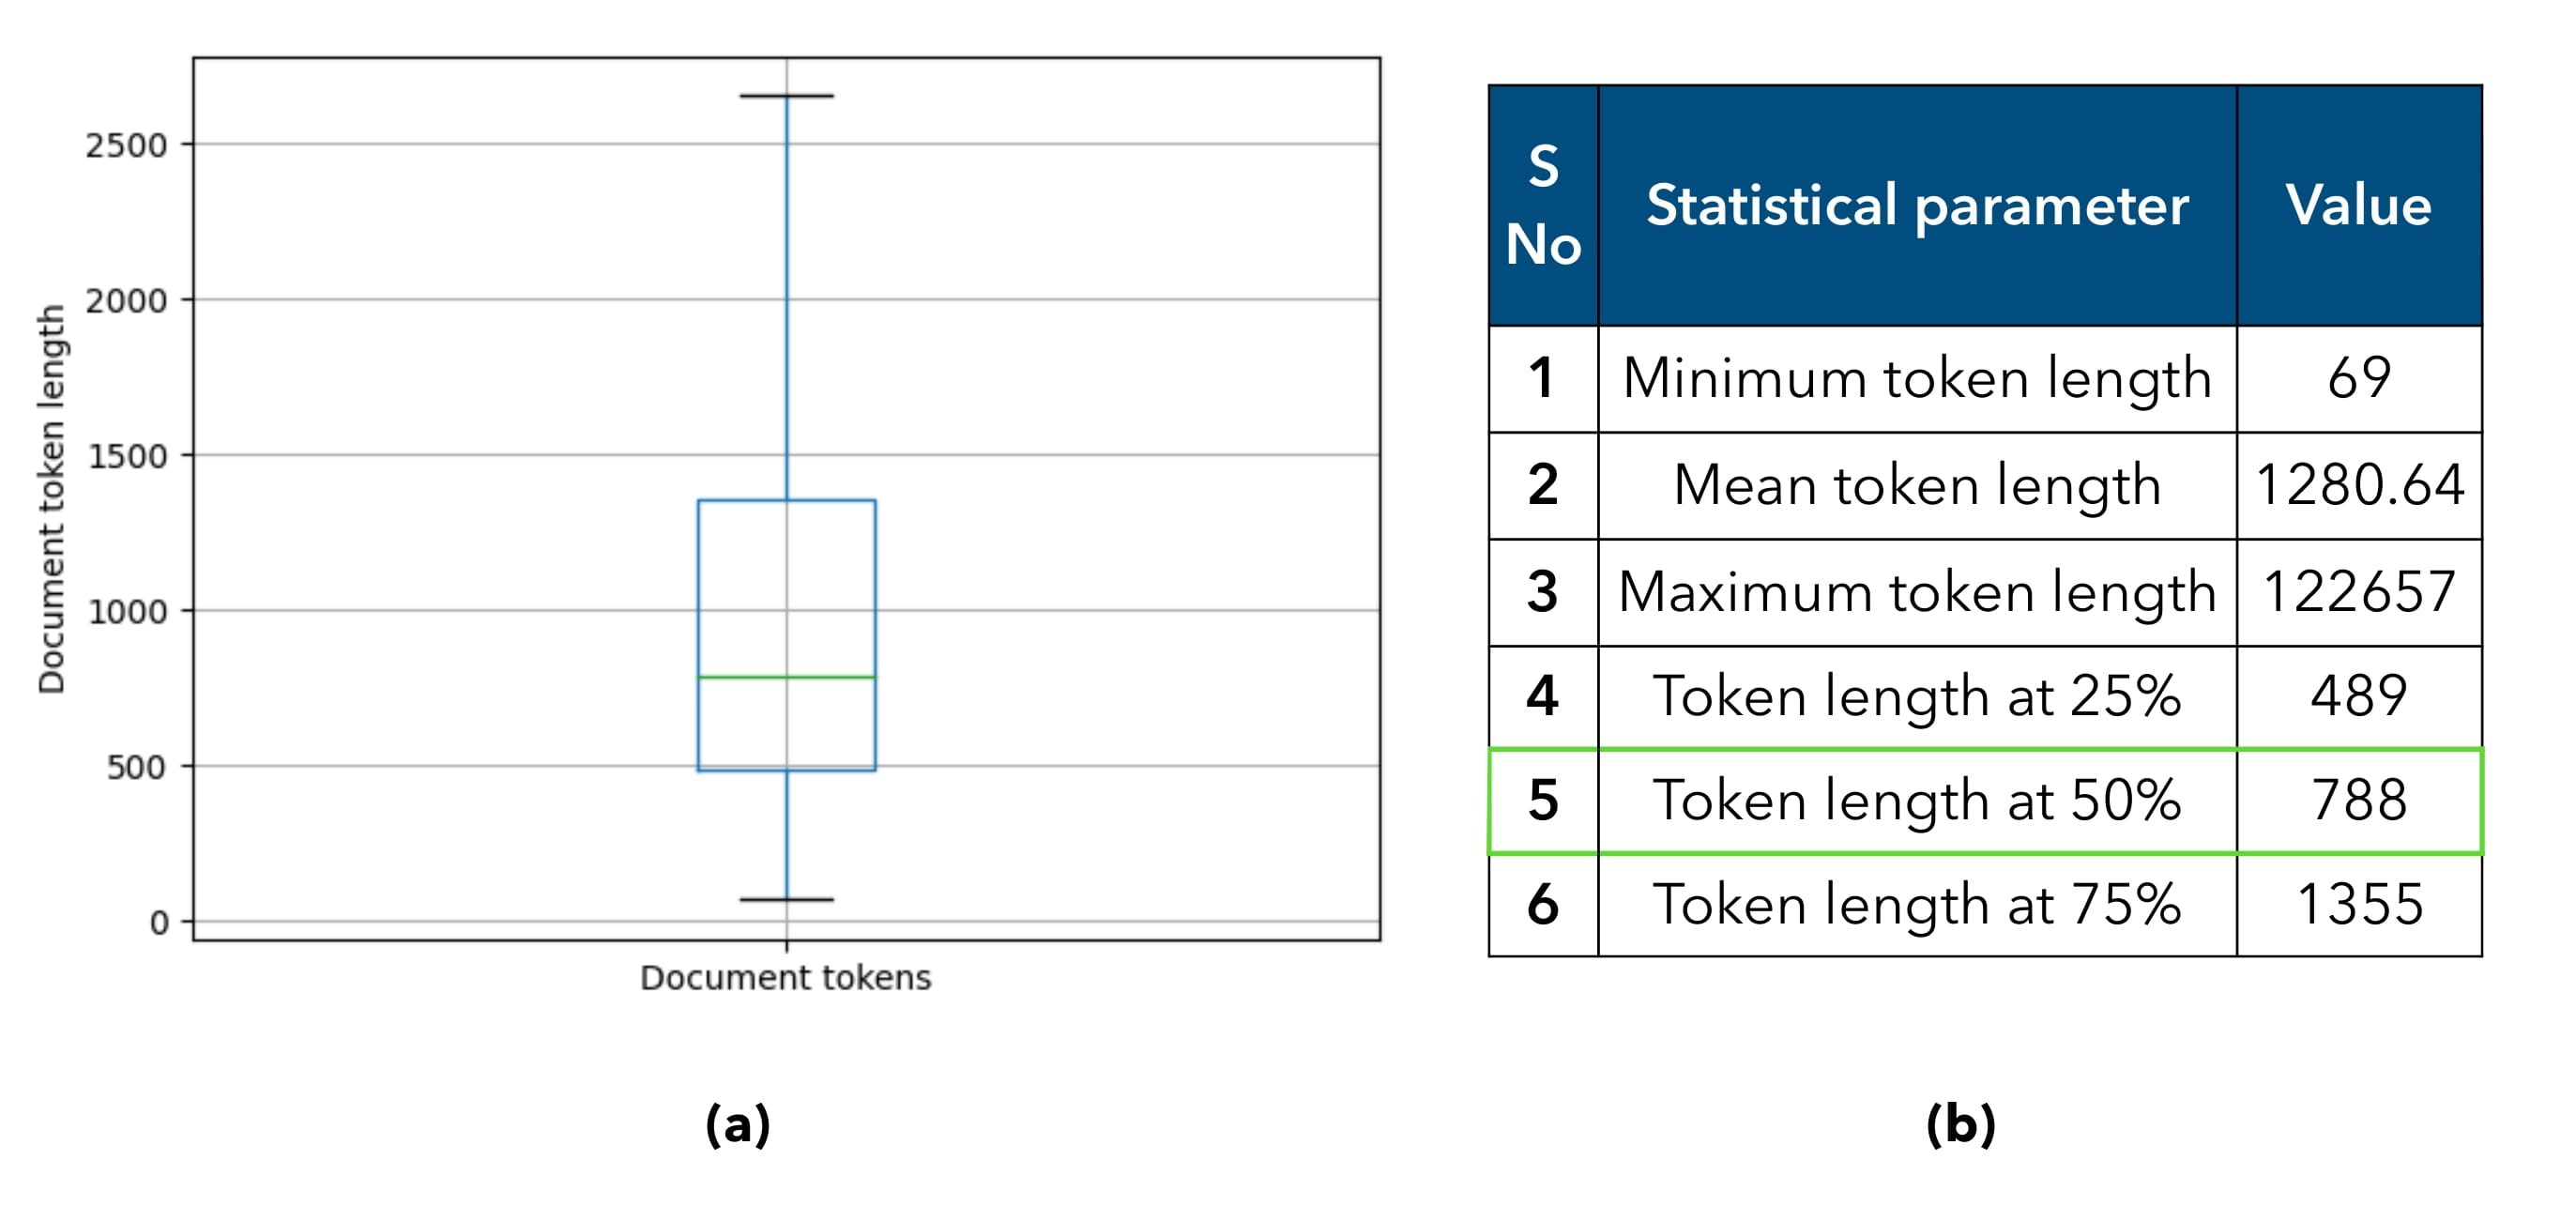
\includegraphics[width=.8\textwidth]{images/keynotes_images/token_length_distribution.jpg}
	\caption{(a) Bloxplot showing the document token length distribution(after removing the outliers) (b) Important statistical details about the token length  \label{fig:token_length_distribution}}
\end{figure}



	Information related to innovation and technological breakthroughs is hard to find in the news articles. However, the probability is not zero, as positive news articles
	are gathered during data collection for classification. Nevertheless, their low distribution makes it challenging to create a dataset sufficient for supervised approaches. After considering the challenges with positive documents for the user intention, a supervised solution is hard to achieve, in order to match the performance of a full sentence query.  Real-time user feedback and continuous reinforcement
	algorithms can fulfill the lack of labeled datasets, but they need feedback from diverse
	users regularly. Otherwise, the search results can be highly inclined to a particular user and
	lead to biased results.
	


A template-based search query is an option to improve the context of a search query. For example, we have a pre-defined template such as \textit{Innovations in XXX related to the Military}. When the user provides a query: \textit{Robotics}, we replace the \textit{XXX} with the user query, and this results in the final query  \textit{Innovations in Robotics related to Military}. An option to update the template according to the user's interest from the user interface can provide tailored results without any extra training. This approach restricts the user to having only a few sets of templates and is also inefficient when a new template needs to be added, or an existing template needs to be updated. 

\begin{figure}[h]
	\centering
	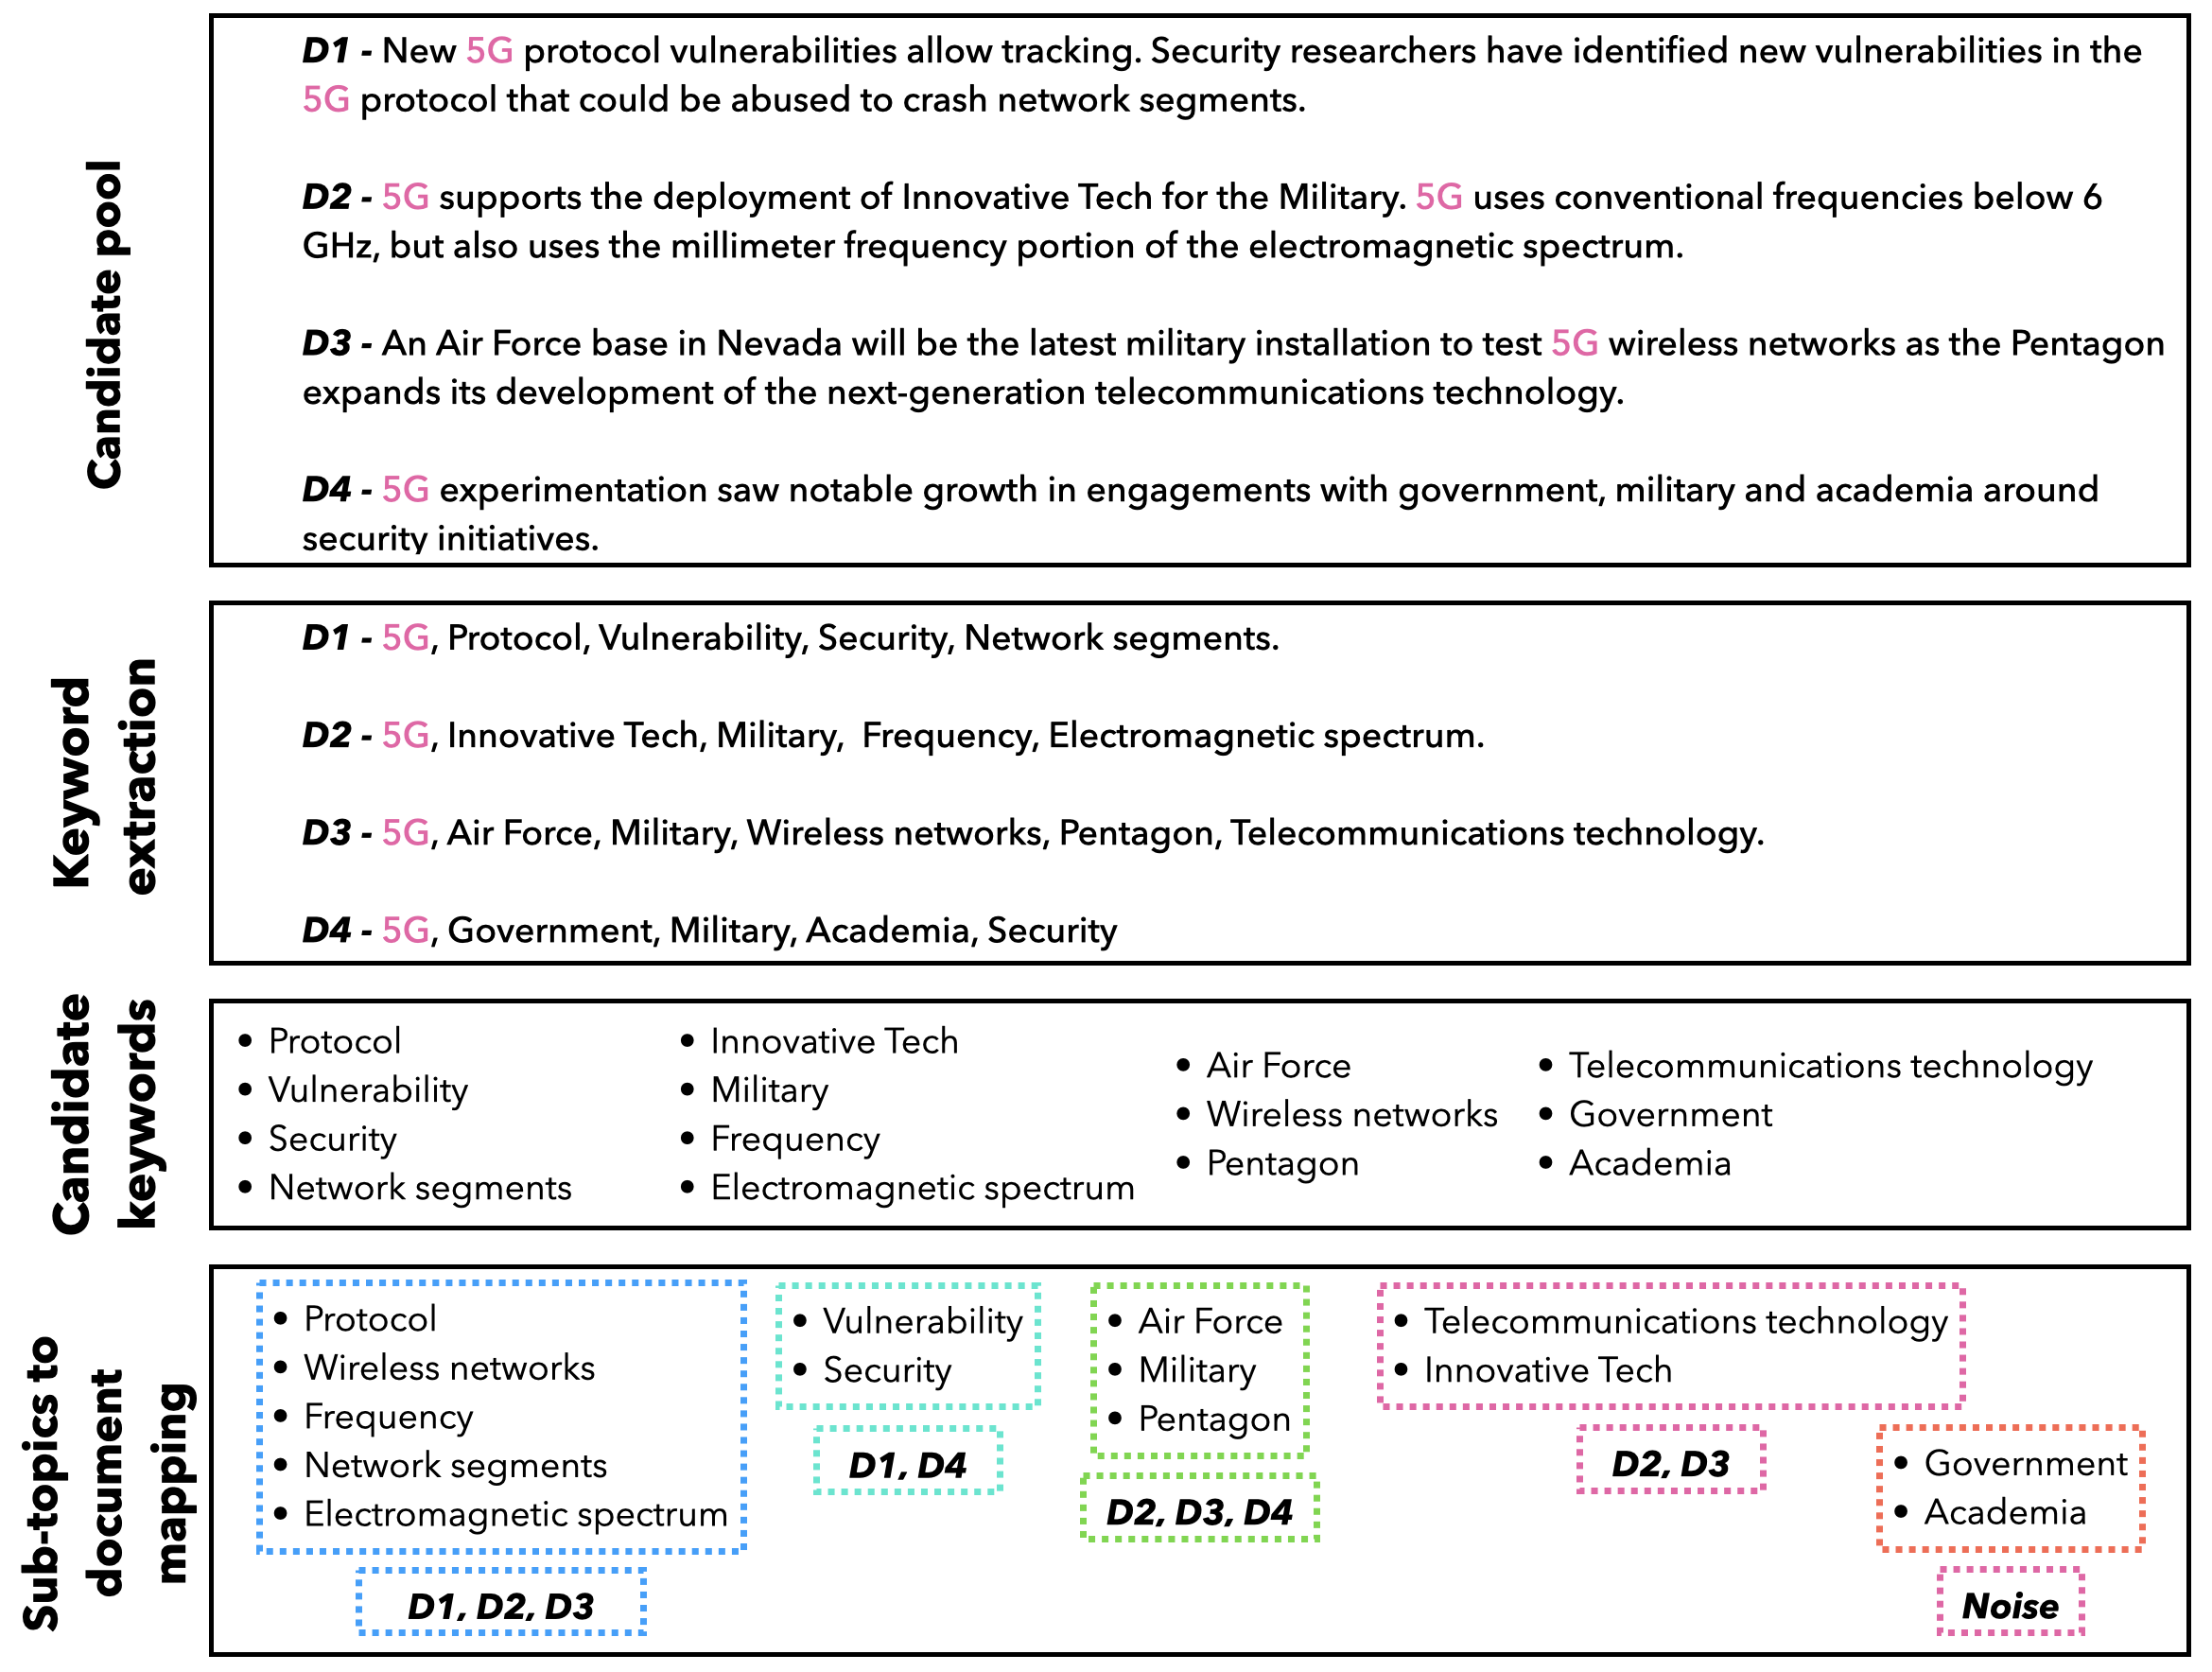
\includegraphics[width=.9\textwidth]{images/keynotes_images/high_level_approach.jpg}
	\caption{Expected sub-topic extraction for the query: 5G \label{fig:proposal_idea}}
\end{figure}

After considering various approaches to fulfill the missing context, we believe that extracting the contexts
from top results to the user query in an unsupervised way is more efficient, more explainable and can be better reproducible compared to supervised approaches. This would not only help the user to have deep insights into the results pool but also reduce the efforts to reach the highly relevant documents. A sample expected sub-topic extraction pipeline output is shown in \prettyref{fig:proposal_idea}. These contexts are described as \textit{sub-topics}.  The proposed approach in this master thesis is aimed at handling the challenges mentioned above. News articles from diverse sources are considered, and the results can be easily transferred to other data sources in the future. 


	\section{Proposed methodology}

One way to extract different contexts from the candidate pool is to perform any clustering
algorithm on the retrieved documents. This results in very generic clusters closely related to a given query and does not provide any new insights to the user. To generate diverse and distinctive clusters, we need to use the latent information at the word or phrase level rather than at the document level~\cite{blei2003latent}. As the documents contain multiple occurrences of the query and are also highly similar in semantic space, we need to reduce the impact of the given user query to generate a clear distinction between the documents. \prettyref{fig:methodology2} illustrates the proposed approach on an abstract level. 

\begin{figure}[h]
	\centering
	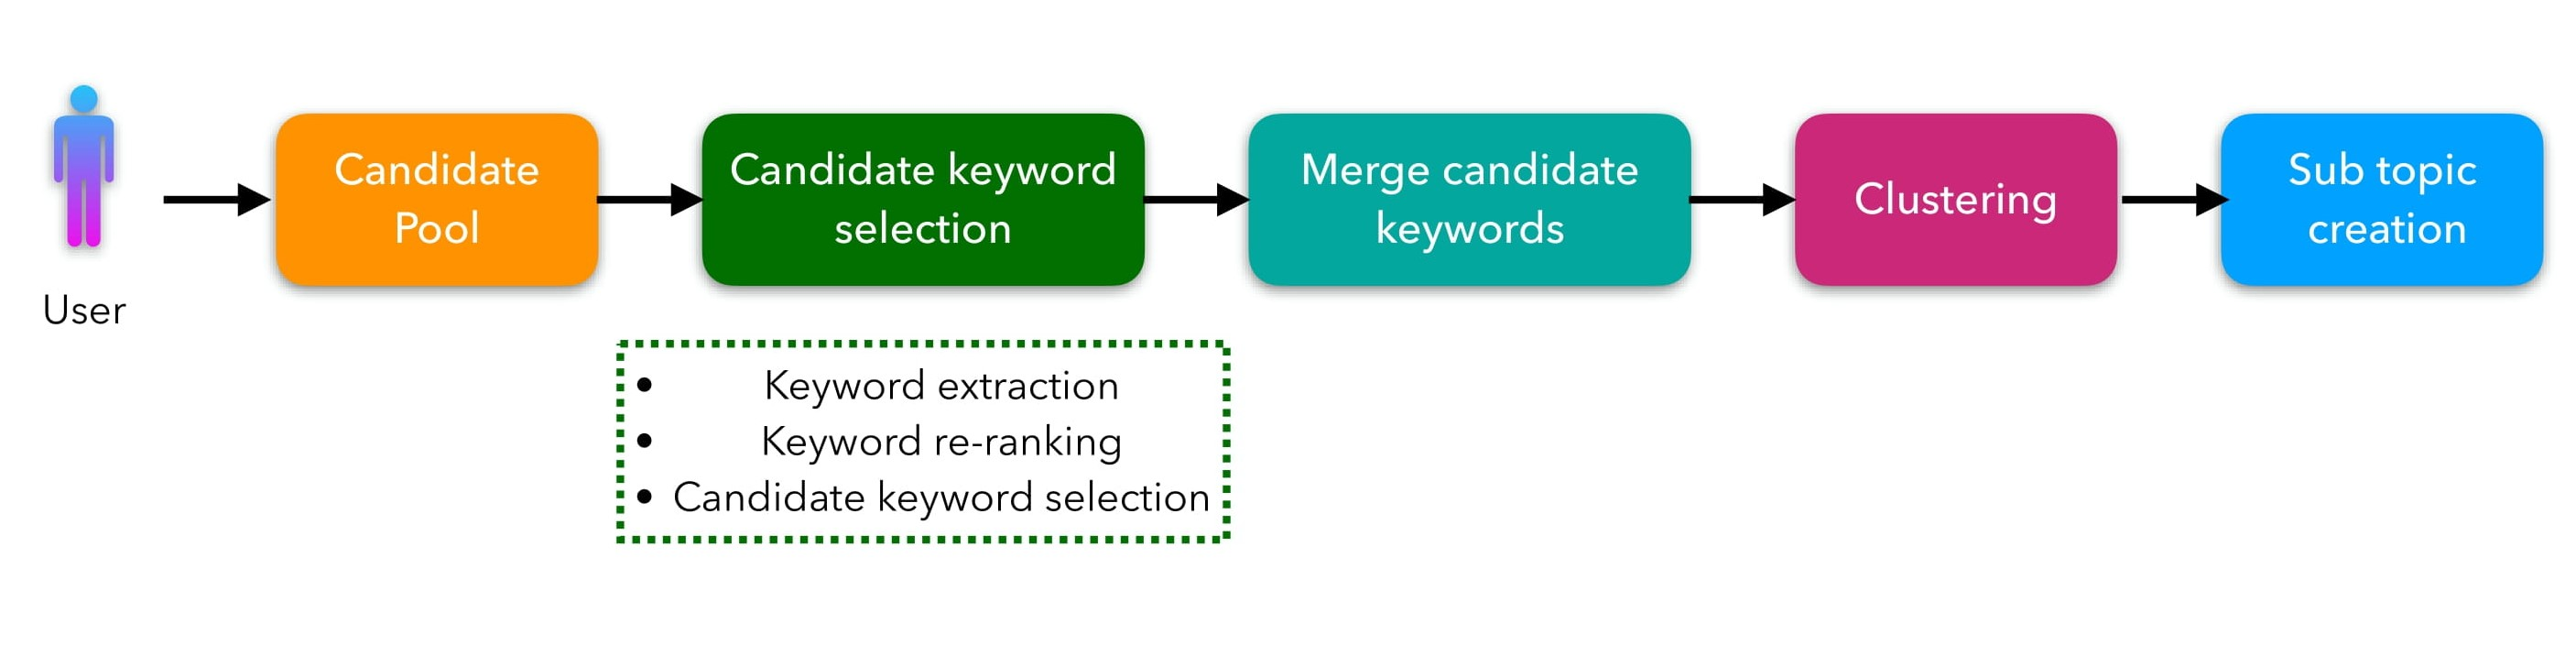
\includegraphics[width=.8\textwidth]{images/keynotes_images/methodology.jpg}
	\caption{Proposed approach on an abstract level \label{fig:methodology2}}
\end{figure}

The proposed approach, shown in \prettyref{fig:methodology2},  does not assume fixed templates or specific user intentions. Major components in the pipeline are: \textit{Candidate keyword selection, Merge candidate keywords, Clustering, and Sub-topic creation}. This pipeline's first step is retrieving a candidate or retrieval pool for the given query. Subsequently, to extract keywords with high diversity and low noise (stopwords), a Candidate selection module is proposed.  This component consists of three significant steps namely \textit{Keyword extraction, Keyword re-ranking}, and \textit{Candidate keyword selection}.

\mycomment{
 Noun chunks are extracted from each document with the help of the Spacy\footnote{\url{https://spacy.io/}} library and are further cleaned to remov. To clean these noun chunks, a pipeline is proposed with the following tasks: \textit{Stopword removal, N-gram range (1, 3), Remove punctuation, Remove determiners, Lemmatization, and Remove noun chunks containing numeric, Remove close duplicates using fuzzy matching}. Cleaned noun chunks are then re-ranked according to the cosine similarity to the original document. Top-k noun chunks with highest cosine similarity is selected and further used in clustering. This process of selecting top noun chunks in a document is named Candidate noun-chunk selection and resulting phrases are referred to as keywords. This approach is inspired from the recent research related to using contextualized sentence embeddings for keyphrase extraction~\cite{bennani2018simple}.}

\begin{figure}[h]
	\centering
	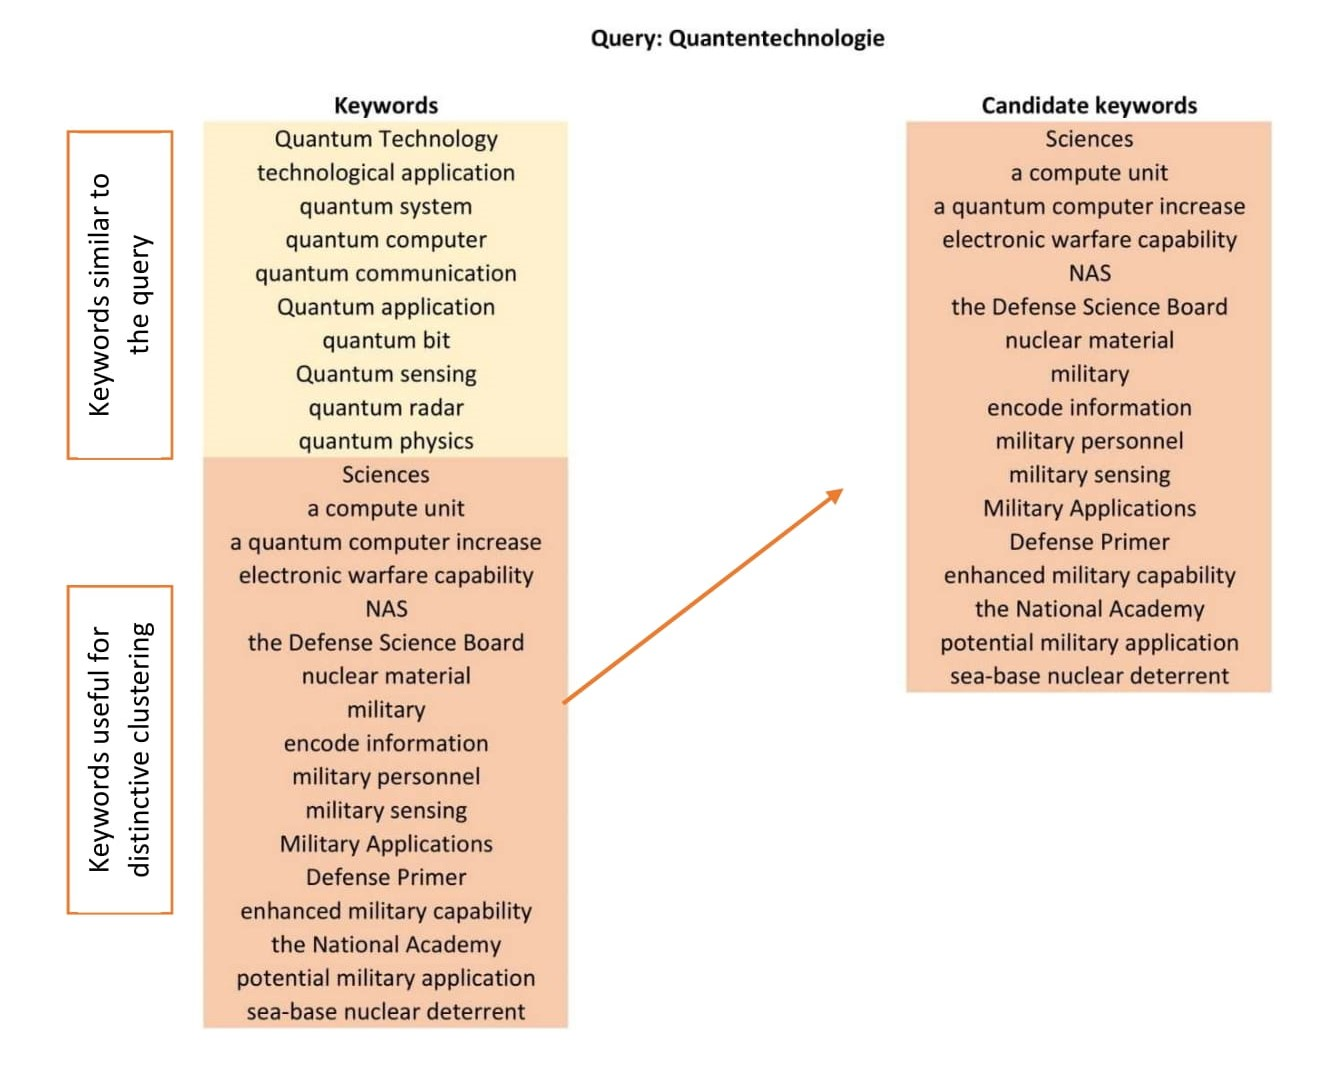
\includegraphics[width=.8\textwidth]{images/keynotes_images/candidate_keywords.jpg}
	\caption{Candidate keyword selection step from a single document \label{fig:candidate_keywords}}
\end{figure}


\textit{Keyword extraction} is extracting the most meaningful  noun phrases in a text document. In the second stage, \textit{Keyword re-ranking}, cosine similarity is calculated from the phrase embeddings between the keywords and the query. Using these similarity scores, keywords are then re-ordered in descending order. After this stage, the certain keyword, that are not similar to the query have a low cosine similarity score are precisely extracted, as they have a high potential for creating distinctive clusters or sub-topics. Specific keywords are selected and used for clustering using a cut-off threshold and this process is referred to as \textit{Candidate keyword selection} and the resulting phrases after this stage are called Candidate keywords, shown in \prettyref{fig:candidate_keywords}.

The second component in the pipeline, \textit{Merge candidate keywords}, merges candidate keywords from each document in the candidate pool and duplicates are removed. These keywords are then clustered semantically and modeled with the documents again. This process is also referred as Document to sub-topic modeling and is designed independent to the query and to handle multiple languages. 

\mycomment{This component has three main steps namely Phrase embeddings, Dimensionality reduction, and Hierarchical clustering. To achieve semantic clustering, multi-lingual contextualized sentence encoders are considered to generate phrase embeddings for each candidate keyword. These densely distributed embeddings are usually highly dimensional (512 or 768) and the clustering in such high dimension is  complex to capture patterns and can be resource intensive. Therefore, the embeddings are compressed with a dimensionality reduction technique. }




\mycomment{Therefore, the dimensionality of the embeddings is reduced without losing underlying information in the data using the UMAP algorithm~\cite{mcinnes2018umap} from the umap-learn library. These embeddings are further clustered in lower dimensions using a hierarchical clustering algorithm. Noise is expected in the candidate keyword extraction phrase and all the keywords are not important for modeling. The clustering algorithms such as k-means, Gaussian Mixture Models, etc., are not suggested in this case, as they consider all data-points while clustering. Consequently, HDBSCAN and DBSCAN clustering algorithms are preferred as they innately consider the noise in the data and avoid assigning a cluster for every data point. One major advantage of these algorithms is that the cluster count is not a parameter and the algorithm creates clusters effectively based on the data. HDBSCAN algorithm~\cite{mcinnes2017hdbscan} with its varying epsilon and merging clusters has shown robust clustering results by finding varying density clusters and the same algorithm is considered in the proposed approach. This clustering pipeline is already tested and shown great results with documents in recent research~\cite{angelov2020top2vec}.
}



After clustering, sub-topics are extracted using a centroid approach. A mean phrase vector (centroid vector) is calculated from all the keywords inside a cluster and the closest keyword vector to the centroid vector is considered a cluster label. This process is named \textit{Cluster labeling} and the cluster labels are considered sub-topics. After clustering, the individual clusters are considered as sub-topics. Sub-topics and documents inside a sub-topic can be further ranked before showing to the user. The pipeline ends with this last component, \textit{Sub-topic creation}. 

\mycomment{Initial pipeline results are shown in \prettyref{fig:subtopic_search}. \prettyref{tab:hyper_parameters} shows the parameters which will be tuned during clustering evaluation.

\begin{center}
	\captionof{table}{Parameters in the model for tuning}\label{tab:hyper_parameters}
	\begin{tabularx}{.7\textwidth}{|c|Y|Y|c|}
		\hline
		S No. & Hyperparameters & Range & Possibilities \\
		\hline
		1 & Candidate keyword selection & [0.3, 0.4, 0.5] & 3 \\
		\hline
		2 & Reduced dimensions (Umap) & [3, 5, 10] & 3 \\
		\hline
		3 & Min cluster size (Hdbscan) & [20, 30, 40, 50 ] & 4 \\
		\hline
		4 & Min samples(Hdbscan) & [1, 3, 5, 7 ] & 4 \\
		\hline
	\end{tabularx}
\end{center}
}
	\section{Evaluation}
	
	\subsection{Testset}
	
	For two main reasons, a dataset specific to this research problem is hard to find in the current IR data repositories. Foremost, the search query needs to be a phrase rather than a sentence. Furthermore, the documents need to be labeled with a specific intention rather than just coherence with the query. The interest at Fraunhofer FKIE is to retrieve the documents related to "Innovation and Technology", and a new testset is collected for this purpose. Below are a few specific areas of interest in news articles that describe the user intention: \textit{Innovation, Technology breakthroughs, Future products, Applied research, New procurement strategies, Artificial Intelligence}. These topics are also described as positive document characteristics because a document is considered positive when it is strongly related to any one of the above-mentioned characteristics. 
	
	\begin{figure}[h]
		\centering
		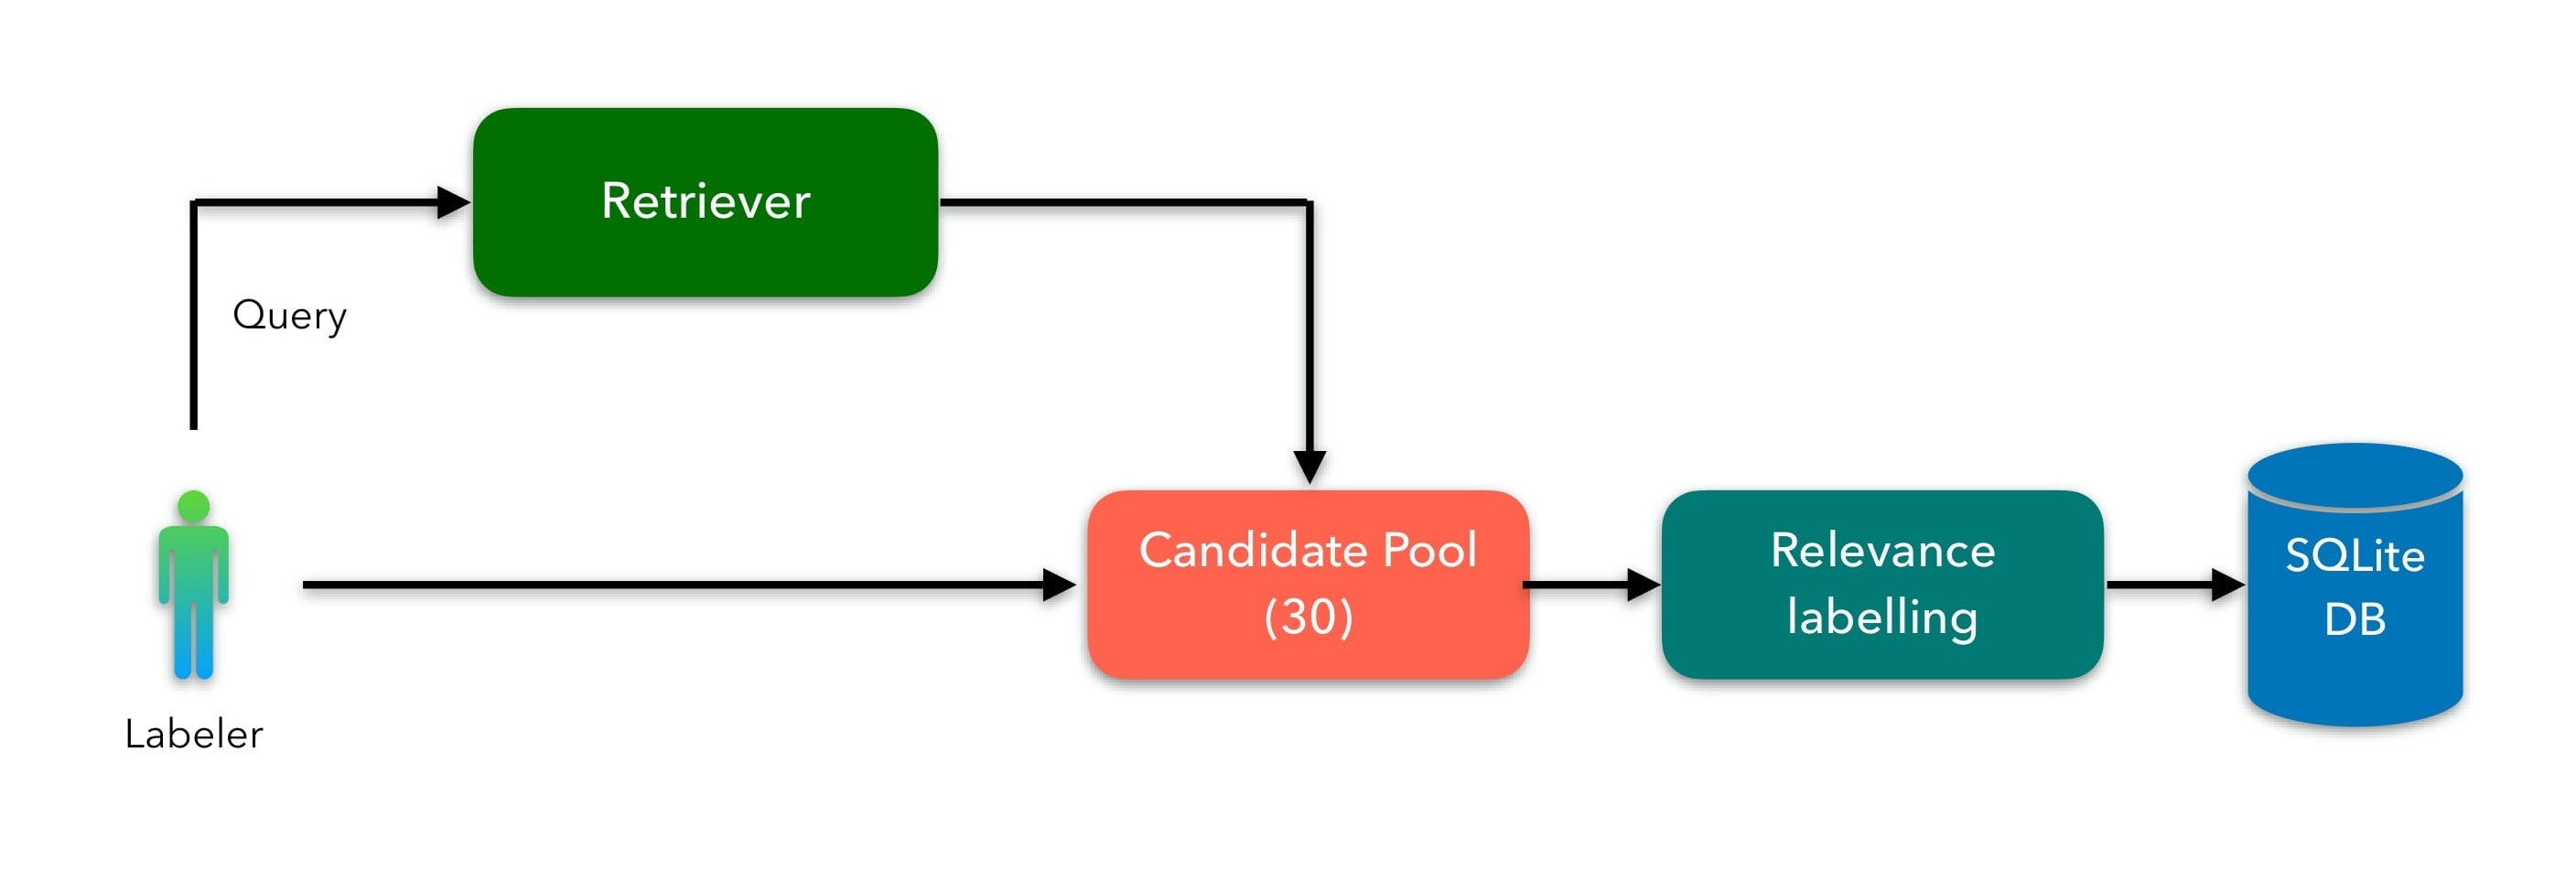
\includegraphics[width=.8\textwidth]{images/keynotes_images/dataset.jpg}
		\caption{Testset collection strategy \label{fig:dataset}}
	\end{figure}
	
The strategy for the testset collection is to consider documents from lexical and semantic
matching. The results from both algorithms help find the diverse contexts
related to the user query. Therefore, a candidate pool with a maximum length of 30 documents
from both lexical and semantic matching is considered. Fifteen documents from the
above search systems are combined to a merged set where duplicate documents are eliminated. The image \prettyref{fig:dataset}
shows the methodology followed for the testset collection. \textit{Relevance labeling}, is a process to assign an appropriate label to the
retrieval results inside the candidate pool. Every labeler has to assign a label not only coherent to
the query but also considering the FKIE user's intention, i.e., coherence with positive document
characteristics mentioned above. Once the labeler assigns a particular label to a document, labeled information is stored in an SQLite DB.\pagebreak
	
	\begin{center}
		\captionof{table}{Relevance label definitions}\label{tab:label_definitions}
		\begin{tabularx}{0.8\textwidth}{|c|c|Y|}
			\hline
			Label-id & Label name &  Label definition \\
			\hline
			1 & Perfect & A document that strongly matches  one of the positive document characteristics. \\
			\hline
			2 & Partially relevant &  A document that contains keywords and seems to be relevant, but still lacks innovation or novelty.\\
			\hline
			3 & Irrelevant &  A document containing the given user keyword still lacks innovation and
			coherent discussion about the query.\\
			\hline
			4 & Wrong & These are false documents and have nothing to do with the user	query.\\
			\hline
		\end{tabularx}
	\end{center}
	
\mycomment{	\begin{figure}[h]
		\centering
		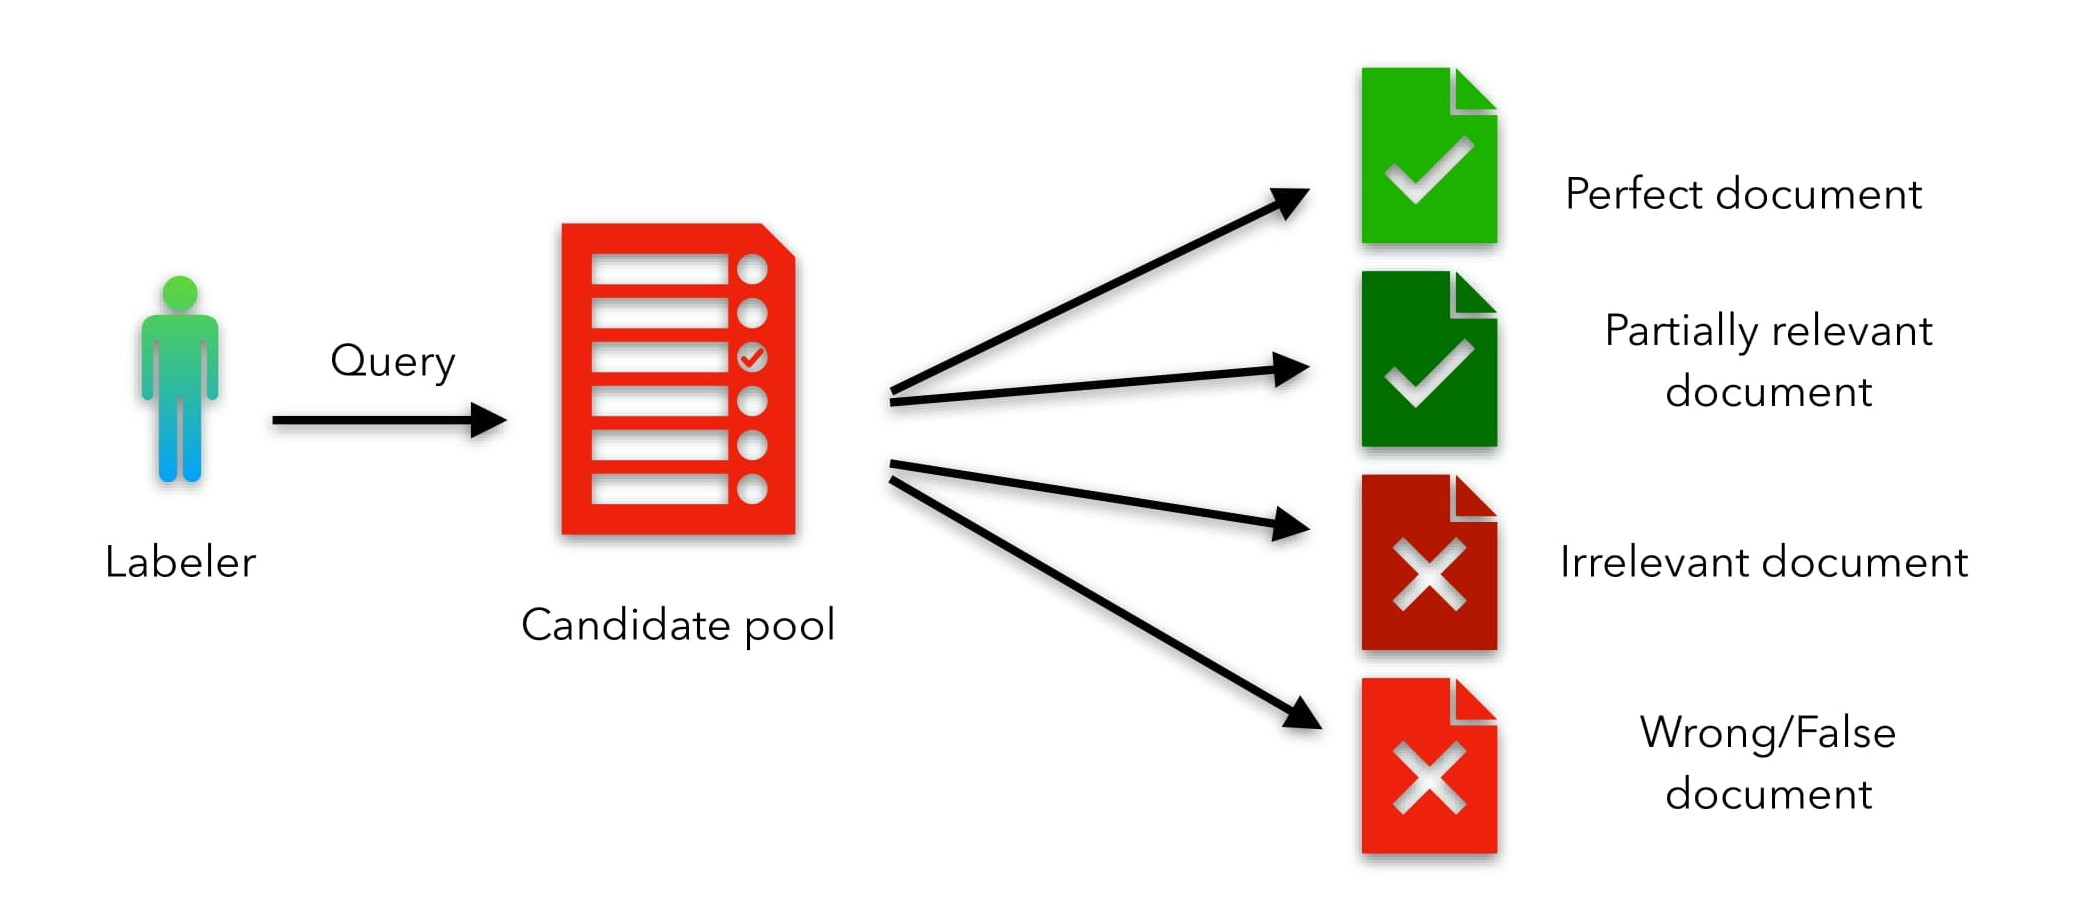
\includegraphics[width=.7\textwidth]{images/keynotes_images/relevance_labeling.jpg}
		\caption{Relevance labeling of the candidate pool \label{fig:relevance_labeling}}
\end{figure}}
	
	\subsection{Clustering evaluation}
	
\mycomment{	In case of no labeled data, the clustering output is generally evaluated using an intrinsic evaluation approach. As described above, a small testset is collected and used for the extrinsic evaluation.  \textit{Silhouette index}~\cite{rousseeuw1987silhouettes} is a target function used for the intrinsic clustering evaluation and is calculated by using the intra-cluster and inter-cluster distances for each sample.} 
	
	 To evaluate the quality of clustering, the  \textit{Silhouette index} is considered for the intrinsic evaluation, and a custom target function $F$ is designed.  Target function $F$ tests the quality of clusters against the relevance labels from the dataset. The objective is to test whether the relevant documents are clustered into a similar cluster and the same case with irrelevant documents. Without any relation between clustering and relevance labeling, it can not be assumed that the positive and negative documents
	 are clustered automatically because they cover a wide range of keywords in different domains. Therefore, it is more meaningful to evaluate the clustering for negative documents, i.e., Irrelevant and Wrong labeled documents. A target function is designed to address
	 the number of negative documents isolated through sub-topic modeling.

\mycomment{\begin{center}
		\captionof{table}{Label distributions in the testset}\label{tab:label_distribution}
		\begin{tabularx}{0.6\textwidth}{|c|Y|c|}
			\hline
			Label-id & Label name & Document count \\
			\hline
			1 & Perfect & 78 \\
			\hline
			2 & Partially relevant & 147 \\
			\hline
			3 & Irrelevant & 306 \\
			\hline
			4 & Wrong & 98 \\
			\hline
		\end{tabularx}
\end{center}}
	
	The sub-topic modeling pipeline's output is distinctive clusters with a unique context, 
	independent of relevance to user intention. However, the clusters can be divided into relevant and irrelevant clusters according to the relevance labels in the dataset.
	Let us consider that $N_1, N_2, N_3, N_4$ represent functions to get the number of documents in a single cluster with label-ids $1, 2, 3, 4$ respectively, as shown in \prettyref{tab:label_definitions},  and $C$ represents the cluster set. 
	
	\centerline{$C$ = $\{c_1, c_2, c_2,\dots\}$}
	
	Relevant clusters $C_r$ are clusters, that contain at least one document with label-id $1$ or documents with majority of label-id $2$. This can be determined using the below expression.
	
	\centerline{$C_r$ = $\{c_i \in C | (N_1(c_i) > 0) \lor (2 * N_2(c_i) >= (N_3(c_i) + N_4(c_i))) $}
	
	With this expression, relevant clusters are differentiated from others and the focus is only on labels $1$ and $2$. The clusters that do not satisfy the above condition are logically considered irrelevant clusters. 
	
	\centerline{$C_i$ = $\{c_j \in C \setminus C_r\} $}
	
	The target function assesses the clustering with a ratio of documents in irrelevant documents to the documents in the candidate pool $CP_q$ to a given user query $q$. Given $N$ queries, the target function maps the score using the below equation. 
	
	\centerline{$F$ = $\sum\limits_{i=1}^N (|C_i|/|CP_i|) * 100 $}
	
	Both the target functions \textit{Silhouette index} and $F$ are used to tune the parameters of the sub-topic modeling pipeline. \textit{Silhouette index} evaluates the clustering output and the custom target function $F$ evaluates the distribution of relevant labels. An automatic parameter tuning can lead to very small clusters and there is a possibility of documents being marked as noise. Therefore,  A manual evaluation of these two metrics will be considered to finalize the pipeline parameters. 
	
	\subsection{Survey evaluation}
	
	The survey proposed evaluates the clustering output and also tests the
	performance of new search query results for a given query and sub-topic. Below two IR systems are proposed and further compared using the survey data.
	
	\begin{enumerate}
		\item 	\textbf{System A} is an IR system that retrieves documents using a new search query based on the original query and the chosen sub-topic.
		
		\item 	\textbf{System B} is an IR system that retrieves documents from the sub-topic clusters from the sub-topic modeling output.
	\end{enumerate}
	
	A new search query strategy still needs to be designed, and
	the number of survey inputs is still being determined.
		
	\subsection{Precision evaluation}
	Assuming that the cluster labels are not very helpful to the user, the next evaluation technique shows that the clustering output does not deteriorate the performance of the retrieval results.
	
	The output of clustering is hard to examine with the baseline IR systems because the order of documents is missing and the actual performance metrics related to false positives are not addressed. For this purpose, we are extending the sub-topic creation with sub-topic ranking and document ranking. These two rankings help the existing pipeline to create a sequential order of documents and facilitate the evaluation of precision against the baselines. Therefore, this evaluation approach proposes six different retrieval systems and evaluates the ranked results. 
	
\begin{center}
\captionof{table}{Proposed IR systems for evaluation}\label{tab:ir_systems}
\begin{tabularx}{0.8\textwidth}{|c|c|c|Y|}
		\hline
		S No. & Flat clusters & Sub-topic ranking & Document ranking \\
		\hline
		1 & IR0 & NA & Uniform distribution \\
		\hline
		2 & IR1 & NA & Query similarity \\
		\hline
		3 & IR2 & Query similarity & Query similarity \\
		\hline
		4 & IR3 & Template similarity & Template similarity \\
		\hline
		5 & IR4 & Document cardinality & Query similarity \\
		\hline
		6 & IR5 & Random combinations & Query similarity \\
		\hline
\end{tabularx}
\end{center}
	
	The first system, \textit{IR0}, is an arbitrary system where the positive documents are distributed uniformly on the ranking order. \textit{IR1} system is simple query re-ranked results based on cosine similarity between the query and documents. The systems \textit{IR2, IR3, IR4} are results of sub-topic
	pipeline clustering, where the clusters are first ranked, and later the documents are re-ranked with
	certain criteria. These three systems simulate the user reading the results linearly or in
	a sequence.  In \textit{IR2}, the sub-topic clusters are ranked by the cosine similarity between the query and centroid vector of the cluster and similarly for document ranking. 
	
	The system \textit{IR3} uses a template similarity criteria, where the similarity is calculated between a template and centroid vector rather than the query. For example, the template string can be "Innovation and Technology". In the same way, \textit{IR4} clusters are ranked using the number of documents in the cluster. The last system, \textit{IR5}, is an unreal system just like the \textit{IR0}, but multiple combinations of random ranking of clusters are considered to simulate the random selection of a sub-topic by the user and reading the documents in different sub-topics. 
	
	In ~\cite{mehlitz2007new}, a new evaluation measure for IR systems named expectation score is introduced. The Expectation score ($E$) is similar to Precision ($P$) but does not consider false positives. $E_k$ represents the number of positive documents at the index k, whereas $P_k$ represents the ratio of positive documents at the index k to k. Furthermore, Mean Average Precision (MAP)~\cite{cormack2006statistical} is used to evaluate the ranking performance. MAP is calculated through the Average Precision (AP) metric, which is an average of precision scores only at the positive document indices. Let us consider that $G$ is a set of all positive document index with size $g$. 
	
	\centerline{$AP$ = ($\sum\limits_{i=1}^G P_i) /g$}
	
	\centerline{$MAP$ = ($\sum\limits_{i=1}^N AP_i) /N$}
	
	
	\subsection{Evaluation summarization}
	
	The table \prettyref{tab:evaluation_rq} shares the evaluation techniques chosen in this thesis and the respective research questions answered.
	
	\begin{center}
		\captionof{table}{Proposed evaluation techniques }\label{tab:evaluation_rq}
	\begin{tabularx}{0.7\textwidth}{|c|c|Y|}
		\hline
		S No. & Evaluation type & Research questions addressed \\
		\hline
		1 & Clustering  & \textbf{RQ1} \\
		\hline
		2 & Survey  & \textbf{RQ1, RQ2} \\
		\hline
		3 & Precision analysis & \textbf{RQ3} \\
		\hline
	\end{tabularx}
\end{center}

\section{Work Packages with Schedule}

Work packages with deadlines is shown in ~\prettyref{fig:work_packages}

\mycomment{\begin{center}
		\captionof{table}{Work packages with date deadlines  }\label{tab:work_packages_table}
		\begin{tabularx}{0.99\textwidth}{|c|Y|c|c|c|}
			
			\hline
			S No. & Work package & Start date & End date & Duration (in days) \\
			\hline
			1 & Candidate pool strategy implementation & 23.1.23 & 24.1.23 & 2 \\
			\hline
			2 & Candidate selection pipeline implementation & 25.1.23 & 27.1.23 & 3 \\
			\hline
			3 & Clustering and complete pipeline testing & 30.1.23 & 10.2.23 & 10 \\
			\hline
			4 & Baseline and IR system development & 13.2.23 & 17.2.23 & 5 \\
			\hline
			5 & Expectation score and precision analysis & 20.2.23 & 27.2.23 & 6 \\
			\hline
			6 & Mid-term presentation & 28.2.23 & 28.2.23 & 1 \\
			\hline
			7 & Survey development with UI and data collection & 1.3.23 & 10.3.23 & 8 \\
			\hline
			8 & Survey analysis and results evaluation & 13.3.23 & 17.3.23 & 5 \\
			\hline
			9 & Final report for review (and further analysis) & 20.3.23 & 21.4.23 & 25 \\
			\hline
			10 & Final report submission & 24.4.23 & 19.5.23 & 20 \\
			\hline
			
		\end{tabularx}
\end{center}}


	\begin{figure}[h]
	\centering
	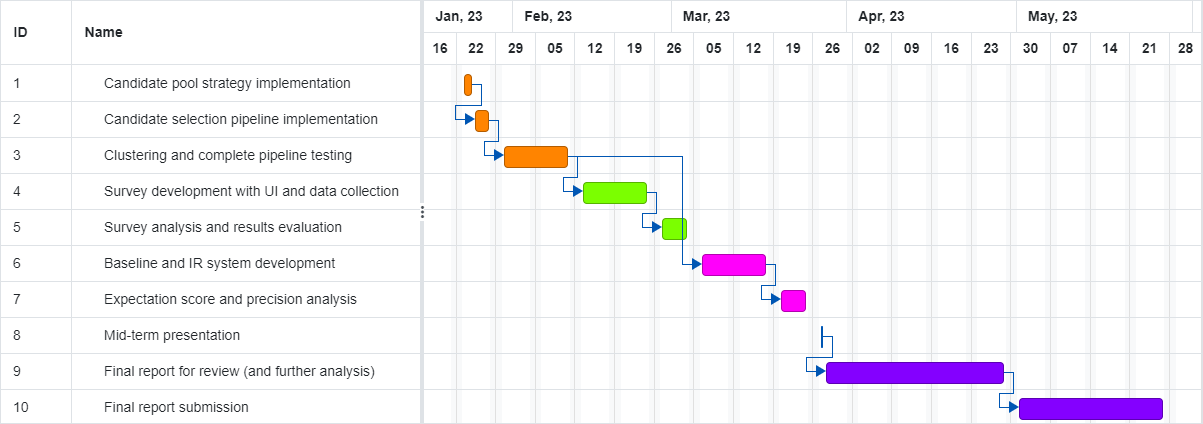
\includegraphics[width=.8\textwidth]{images/work_packages_schedule.png}
	\caption{Work packages and schedule \label{fig:work_packages}}
\end{figure}
	
	
\section{Scientific background}

Many researchers have considered different techniques from Machine Learning (ML) to improve the retrieval results based on the availability of labeled data. The research can be categorized into two types: supervised and unsupervised.

\subsection{Supervised approaches}

 Many researchers used ML algorithms with special loss functions based on relevance between the query, and documents and some of the popular pairwise ranking methods are RankBoost~\cite{freund2003efficient}, RankNet~\cite{burges2005learning}, Rank-SVM~\cite{joachims2002optimizing} (using click-through data). Recent state-of-the-art supervised approaches are neural re-ranking methods and are based on complex Deep Learning (DL) architectures. Distributed word embeddings combined with the performance of non-linear neural networks have shown remarkable results in improving the performance of retrieval systems by considering semantics~\cite{mitra2017learning, guo2016deep, nogueira2019passage}. 

\subsection{Unsupervised approaches}

These approaches use no-labeled data and re-rank the retrieved results based on the user query and top retrieved documents~\cite{rohatgi2020psu, azad2019query}. One common challenge in these approaches is the user query, which is mostly comprised of only a few keywords~\cite{azad2019query, Kankaria2015QueryET}. To tackle this problem, many
researchers have tested Query Expansion (QE) approaches that partially fill the missing meaning and
context in the query. QE techniques include clustering search results, query filtering, word sense disambiguation, and relevance feedback, etc., ~\cite{azad2019query}. Relevance Feedback is a method of retrieving search results using the original query given by the user and then using the top-k documents for query expansion~\cite{azad2019query}. Researchers have clustered search results in many different ways, such as at the document level, keyphrases, query-specific clustering, etc. ~\cite{bernardini2009full, kurland2008rank, zamir1998web, osinski2005concept, liu2004cluster, liu2006representing}. Typical distance-based clustering algorithms such as k-means are used in some research and also Hierarchical clustering is also tested~\cite{bernardini2009full, mehlitz2007new, yuan2022measurement}, as it is flexible to change the threshold level for cutting the clustering dendrogram in a bottom-up approach. A common drawback in most clustering approaches is mapping a document to a single cluster, which is not logically valid, as a document can contain keywords from different domains. 

\subsection{Uniqueness in the proposed approach}

The approaches based on clustering at the word level ~\cite{bernardini2009full, mehlitz2007new} consider only a single language of retrieval results or corpus and hence cannot be directly implemented on a multi-lingual corpus and does not have any special keyword selection stage. With the advantage of contextual embeddings from sentence encoders, the authors in ~\cite{angelov2020top2vec} made a breakthrough in document clustering with an efficient and explainable topic-modeling approach.  

 In ~\cite{malloci2020text},  authors have used a particular candidate selection approach to filter some phrases from the keyword extraction and a specific noun chunks selection. This pipeline is explicitly used to extract innovation insights from research projects. As the user intention is related to \textit{Innovation} at FKIE is proposed as a unique query-specific candidate keyword selection clustering. Moreover, the documents are semantically mapped to a specific topic, and multiple languages
 are modeled using a single multilingual pre-trained sentence encoder. News articles from multiple languages can be easily integrated into the document indices, and no changes are needed in the clustering pipeline. The proposed approach can be further extended to analyze any corpus containing long text documents for a given phrase or keyword. 


% Literaturverzeichnis
\printbibliography[heading=bibintoc]




\end{document}